\section{Resilient Control Architecture}
\label{S:control}%Nicholas
\begin{figure*}
  \centering
  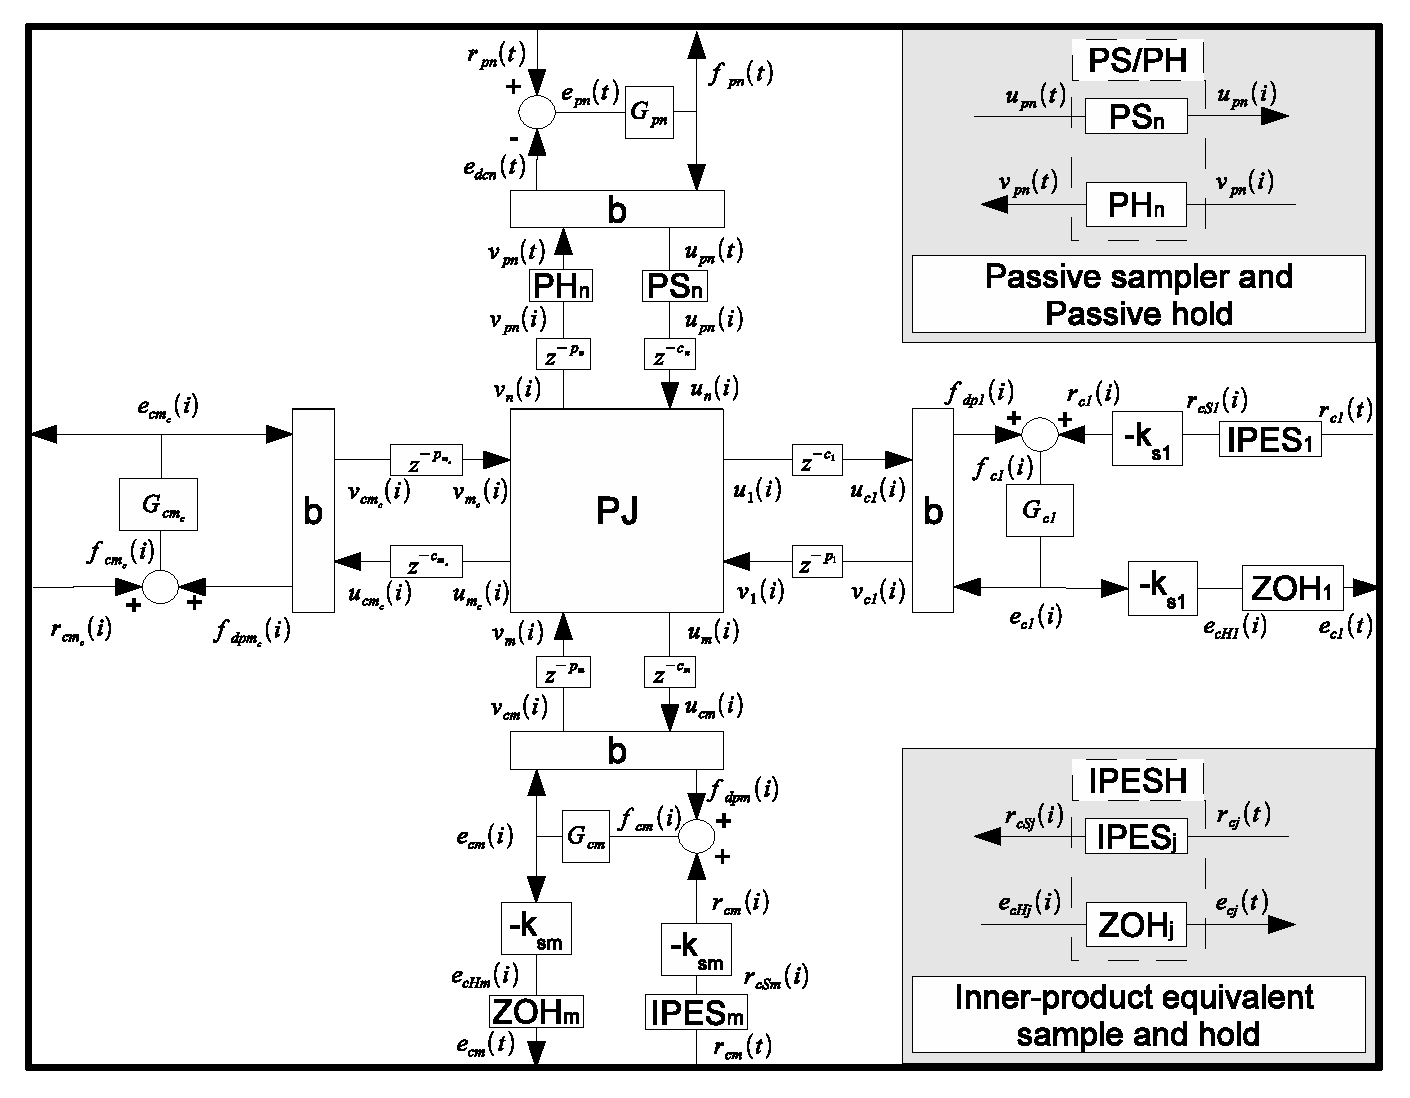
\includegraphics[width=6.0in]{figures/reselient_control_network}
  \caption{An $L^m_2$-stable resilient {\em power junction} control network.}
  \label{fig:resilient_control_net}
\end{figure*}
Fig.~\ref{fig:resilient_control_net} depicts a resilient digital
control network which maintains $L^m_2$-stability, even when
non-redundant controllers could be potentially introduced into the
network.  In particular, $\mathsf{m}$ redundant passive digital
controllers (denoted $G_{\mathsf{cj}}:f_{\mathsf{cj}} \rightarrow
e_{\mathsf{cj}}$ $\mathsf{j}\ \in\ \{1,\dots,\mathsf{m}\}$) and
$\mathsf{m_c} - \mathsf{m}$ non-redundant digital controllers
$\mathsf{j}\ \in\ \{\mathsf{m}+1,\dots,\mathsf{m_c}\}$ are
interconnected to a {\em resilient power  junction} (denoted by the
symbol \textsf{PJ} ) in order to
provide reliable control for a single continuous time 
plant (denoted $G_{\mathsf{pn}}: e_{\mathsf{pn}} \rightarrow
f_{\mathsf{pn}}$ in which $\mathsf{n}=\mathsf{m_c}+1$).  The {\em
  resilient power junction} can be operated in a manner in which it
does not explicitly detect non-redundant controllers or it can
operate in a more-restricted environment in which it enforces that
only redundant controllers can modify the behavior of the plant.
In the more-restrictive mode, non-redundant controllers shall be
isolated from the network so as not to potentially destabilize the
rest of the network.  In regards to notation, we refer the reader to
\eqn{E:ps_ph_cor}, the final form of \eqn{E:ps_ph_cor}, allows us to
simplify numerous expressions which require either integrals or
summations.  More specifically $\innerprod{y}{u}_X$ represents the
inner-product between the two variables $y,\ u$, if $X=N$ ($X=NT_s$) then the
inner-product refers to the discrete-time (continuous-time)
inner-product, in addition the respective squared two-norm
$\twonorm{u}^2=\lim_{X \rightarrow \infty}\twonorm{(u)_X}^2=\innerprod{u}{u}_X$.
\subsection{Wave Variables}
\label{S:wave_variables}
 Networks of a \passive\ plant and controller are typically
  interconnected using {\it power variables}.  {\it Power variables}, 
  denoted by an {\it effort} and {\it flow} pair ($e_*$,$f_*$),
  product is power.  They are typically used to show the 
  exchange of energy between two systems using {\it bond graphs}
  \cite{breedveld06:_port_based_model_dynam_system, golo03:_hamil}.
  However, when {\it power variables} are subject to delays the
  communication channel ceases to be \passive\ which can lead to
  instabilities.  Using a bilinear-transform, the power variables can
  be transformed into wave-variables
  \cite{anderson92:_asymp_stabil_for_force_reflec,
    niemeyer04:_telem}.
\begin{align}
  \label{E:wave_transform_master_u}
  u_{\mathsf{pn}}(t) &= \frac{1}{\sqrt{2b}}(b f_{\mathsf{pn}}(t) + e_{\mathsf{dcn}}(t))\\
  \label{E:wave_transform_master_v}
  v_{\mathsf{pn}}(t) &= \frac{1}{\sqrt{2b}}(b f_{\mathsf{pn}}(t) - e_{\mathsf{dcn}}(t)) 
\end{align}
\begin{align}
  \label{E:wave_transform_slave_v}
  v_{\mathsf{cj}}(i) &= \frac{1}{\sqrt{2b}}(b f_{\mathsf{dpj}}(i) - e_{\mathsf{cj}}(i)),\ \mathsf{j} \in
  \{1, \dots, \mathsf{m_c}\}\\
  \label{E:wave_transform_slave_u}
  u_{\mathsf{cj}}(i) &= \frac{1}{\sqrt{2b}}(b f_{\mathsf{dpj}}(i) + e_{\mathsf{dpj}}(i))
\end{align}
  The wave variable $u_{\mathsf{pn}}$, described by \eqn{E:wave_transform_master_u}, can
  be thought of as the sensor output for plant $G_{\mathsf{pn}}$.
  Analogously the wave variable $v_{\mathsf{cj}}$, described by
  \eqn{E:wave_transform_slave_v}, can be thought of as each actuator
  output for each controller $G_{\mathsf{cj}},\ \mathsf{j} \in
  \{1,\dots,\mathsf{m_c}\}$.  The symbol $i \in \{0,1,\dots\}$ depicts
  discrete time for the controllers, and the symbol $t \in \mathbb{R}$
  denotes continuous time and the two are related to the sample and
  hold time ($T_s$) such that $t=iT_s$.  \eqn{E:wave_transform_master_u} and \eqn{E:wave_transform_master_v} respectively satisfy the following equality:
\begin{equation}
\label{E:wave_transform_master_uv}
\frac{1}{2}(u_{\mathsf{pn}}\tr (t)u_{\mathsf{pn}}(t) - v_{\mathsf{pn}}\tr (t) v_{\mathsf{pn}}(t)) = f_{\mathsf{pn}}\tr (t) e_{\mathsf{dcn}}(t)
\end{equation}
Similarly, \eqn{E:wave_transform_slave_v} and \eqn{E:wave_transform_slave_u} respectively satisfy the following equality $\forall\ \mathsf{j} \in \{1,\dots,\mathsf{m_c}\}$:
\begin{equation}
\label{E:wave_transform_slave_uv}
\frac{1}{2}(u_{\mathsf{cj}}\tr (i)u_{\mathsf{cj}}(i) - v_{\mathsf{cj}}\tr (i) v_{\mathsf{cj}}(i)) = f_{\mathsf{dpj}}\tr (i) e_{\mathsf{cj}}(i).
\end{equation}

  Denote $I \in 
  \mathbb{R}^{m_s \times m_s}$ as the identity matrix.  When
  implementing the wave variable transformation the continuous time
  plant ``outputs''  $(u_{\mathsf{pn}}(t),e_{\mathsf{dcn}}(t))$ are related to the corresponding ``inputs''
  $(v_{\mathsf{pn}}(t),f_{\mathsf{pn}}(t))$ as follows (Fig.~\ref{fig:resilient_control_net}):
\begin{equation}
\label{E:plant_wave_transform}
\begin{bmatrix}
u_{\mathsf{pn}}(t)\\
e_{\mathsf{dcn}}(t)
\end{bmatrix} =
\begin{bmatrix}
-I & \sqrt{2b}I\\
-\sqrt{2b}I & bI
\end{bmatrix}
\begin{bmatrix}
v_{\mathsf{pn}}(t)\\
f_{\mathsf{pn}}(t)
\end{bmatrix}
\end{equation}
 Next, the discrete time controller ``outputs'' $(v_{\mathsf{cj}}(i),f_{\mathsf{dpj}}(i))$ are related to the
  corresponding ``inputs'' $(u_{\mathsf{cj}}(i),e_{\mathsf{cj}}(i))$ as follows (Fig.~\ref{fig:resilient_control_net}): 
\begin{equation}
\label{E:controller_wave_transform}
\begin{bmatrix}
v_{\mathsf{cj}}(i)\\
f_{\mathsf{dpj}}(i)
\end{bmatrix} =
\begin{bmatrix}
I & -\sqrt{\frac{2}{b}}I\\
\sqrt{\frac{2}{b}}I & -\frac{1}{b}I
\end{bmatrix}
\begin{bmatrix}
u_{\mathsf{cj}}(i)\\
e_{\mathsf{cj}}(i)
\end{bmatrix}
\end{equation}

 The {\em power junction} indicated in Fig.~\ref{fig:resilient_control_net} by
  the symbol \textsf{PJ} has waves entering and leaving the power
  junction as indicated by the arrows.  Waves leaving the controllers $v_{\mathsf{cj}}$
  and entering the power junction $v_{\mathsf{j}}$ in which
  $\mathsf{j} \in \{1,\dots,\mathsf{m_c}\}$ have the following
  relationship
\begin{equation*}
v_{\mathsf{j}}(i) = v_{\mathsf{cj}}(i-p_{\mathsf{j}}(i))
\end{equation*}
in which $p_{\mathsf{j}}(i)$ denotes the time delay in transmitting the
control wave from 'controller-$\mathsf{j}$' to the power junction.
Next, the input wave to the plant $v_{\mathsf{pn}}$ is a delayed version of the
  outgoing wave from the {\em power junction} $v_{\mathsf{n}}$ such that 
\begin{equation*}
v_{\mathsf{pn}}(i) = v_{\mathsf{n}}(i-p_{\mathsf{n}}(i))
\end{equation*}
in which $p_{\mathsf{n}}(i)$ denotes the discrete time delay in
transmitting the outgoing wave to 'plant-$\mathsf{n}$'.
Fig.~\ref{fig:resilient_control_net} depicts fixed time
delays using the z-transform (i.e. $z^{-p_{\mathsf{n}}}$).  Next, the outgoing wave from
the plant $u_{\mathsf{pn}}$ is related to the wave entering the power junction
$u_{\mathsf{n}}$ as follows:
\begin{equation*}
u_{\mathsf{n}}(i) = u_{\mathsf{pn}}(i-c_{\mathsf{n}}(i))
\end{equation*}
in which $c_{\mathsf{n}}(i)$ denotes the discrete time delay in
transmitting the wave from 'plant-$\mathsf{n}$' to the power junction.  Last, the input
wave to the controller $u_{\mathsf{cj}}$ is a delayed version of the outgoing
wave from the {\em power junction} $u_{\mathsf{j}},\ \mathsf{j} \in \{1,\dots,\mathsf{m_c}\}$ such
that 
\begin{equation*}
u_{\mathsf{cj}}(i) = u_{\mathsf{j}}(i-c_{\mathsf{j}}(i)),\ \mathsf{j} \in \{1,\dots,\mathsf{m_c}\}
\end{equation*}
in which $c_{\mathsf{j}}(i)$ denotes the discrete time delay in
transmitting the wave from the power junction to
'controller-$\mathsf{j}$' (the delays are denoted as
$z^{-c_{\mathsf{j}}}$ in Fig.~\ref{fig:resilient_control_net}).
\subsection{Passive Sampler and Passive Hold}
\label{S:ps_ph}
In \cite{kottenstette08:_passiv_based_desig_of_wirel}
it is shown how a passive sampler (\PS) a passive hold (\PH) in
conjunction with a \ipes\ (\IPES) and zero-order-hold  (\ZOH) can be
used to achieve a $L^m_2$-stable system consisting of (a) passive robot(s)
and (a) digital controller(s).  The \PS\ and \PH\ framework, unlike
other data-reduction techniques used in telepresence systems  \cite{hirche07:_trans_data_reduc_in_networ_ii}, does
not require the user to take digital waves and convert them back to a 
continuous-time signal to be connected to a continuous-time
controller.   As can be seen in Fig.~\ref{fig:resilient_control_net}
we have connected the \PS\ and \PH\ to plant-$\mathsf{n}$, while
connecting the (\IPES)  and zero-order-hold (\ZOH) block to each
passive digital controller $G_{\mathsf{cj}},\ \mathsf{j}\ \in\
\{1,\dots,\mathsf{m}\}$ in order to relate $r_{\mathsf{cj}}(i)$ to
$r_{\mathsf{cj}}(t)$ and $e_{\mathsf{cj}}(i)$ to $e_{\mathsf{cj}}(t)$
in a passivity preserving manner.  Therefore we recall the following
set of definitions:
\begin{definition}
\label{D:ps_ph}
The passive sampler denoted (\textsf{PS}$_{\mathsf{n}}$) and the
corresponding passive hold denoted (\textsf{PH}$_{\mathsf{n}}$) must
be implemented such that the following inequality is satisfied
$\forall N > 0$:
\begin{eqnarray}
\label{E:ps_ph}
\int_0^{NT_s} (u_{\mathsf{pn}}\tr(t)u_{\mathsf{pn}} (t) - v_{\mathsf{pn}}\tr(t)v_{\mathsf{pn}} (t)) dt -& \nonumber \\
 \sum_{i=0}^{N-1} (u_{\mathsf{pn}}\tr(i)u_{\mathsf{pn}} (i) - v_{\mathsf{pn}}\tr(i)v_{\mathsf{pn}} (i)) \geq& 0.
\end{eqnarray}
\end{definition}
One way to implement the \PS\ and \PH\ is to use the 
{\em averaging passive sampler and hold}.
\begin{definition}
\label{D:avg_ps_ph}
The {\em averaging passive sampler} denoted (\textsf{PS}$_{\mathsf{n}}$) and the corresponding {\em averaging  passive hold} denoted (\textsf{PH}$_{\mathsf{n}}$) is implemented such that for each $l^{\mathrm{th}}$ component ($l \in \{1,\dots,m_s\}$) of the discrete-time-sampled wave $u_{\mathsf{pn}}(i) \in \mathbb{R}^{m_s}$ (denoted $u_{\mathsf{pn}_l}(i)$) is determined from the respective $l^{\mathrm{th}}$ component of the continuous-time wave $u_{\mathsf{pn}}(t) \in \mathbb{R}^{m_s}$ (denoted $u_{\mathsf{pn}_l}(t)$) using \textsf{PS}$_{\mathsf{n}}$ as follows:
\begin{equation}
\label{E:avg_ps}
u_{\mathsf{pn}_l}(i) = \sqrt{\int_{(i-1)T_s}^{iT_s}u_{\mathsf{pn}_l}^2(t) dt}\ \sgn{\int_{(i-1)T_s}^{iT_s}u_{\mathsf{pn}_l}(t) dt}
\end{equation}
and the continuous-time wave $v_{\mathsf{pn}}(t) \in \mathbb{R}^{m_s}$ is determined from the discrete-time wave $v_{\mathsf{pn}}(i) \in \mathbb{R}^{m_s}$ in terms of each of their respective $l^{\mathrm{th}}$ components using \textsf{PH}$_{\mathsf{n}}$ as follows:
\begin{equation}
\label{E:avg_ph}
v_{\mathsf{pn}_l}(t) = \frac{1}{\sqrt{T_s}}v_{\mathsf{pn}_l}(i),\ t \in\ [iT_s,(i+1)T_s).
\end{equation}
\end{definition}
Using a \PS\ and \PH\ such as the {\em averaging passive sampler and
  hold} we can now relate continuous time variables to discrete time
wave variables associated with plant $G_{\mathsf{pn}}$.  Substituting
\eqn{E:wave_transform_master_uv} into \eqn{E:ps_ph} results in the
following inequality for the plant
\begin{equation}
\label{E:ps_ph_p}
\int_0^{NT_s}  f_{\mathsf{pn}}\tr (t) e_{\mathsf{dcn}}(t) \geq \sum_{i=0}^{N-1} (u_{\mathsf{pn}}\tr(i)u_{\mathsf{pn}}(i) - v_{\mathsf{pn}}\tr(i)v_{\mathsf{pn}}(i)).
\end{equation}
If we assume that the networking time delays of the transmission and
reception of the wave variables satisfy
Proposition~\ref{P:passive_t_d_con} (see
Appendix~\ref{S:wave_vars_time_delay}) then the following inequalities hold:
\begin{align}
\label{E:uv_pn_pj}
\twonorm{(u_{\mathsf{pn}})_N}^2 - \twonorm{(v_{\mathsf{pn}})_N}^2 \geq& 
\twonorm{(u_{\mathsf{n}})_N}^2 - \twonorm{(v_{\mathsf{n}})_N}^2\\
\label{E:uv_cj_pj}
\twonorm{(u_{\mathsf{j}})_N}^2 - \twonorm{(v_{\mathsf{j}})_N}^2 \geq& 
\twonorm{(u_{\mathsf{cj}})_N}^2 - \twonorm{(v_{\mathsf{cj}})_N}^2
\end{align}

This leads us to the following corollary which relates \eqn{E:ps_ph_p} to the corresponding pair of waves entering and leaving the {\em power junction} $(u_{\mathsf{n}}(i),v_{\mathsf{n}}(i))$.
\begin{corollary}
\label{C:ps_ph_cor}
The continuous time plant-$\mathsf{n}$ (flow $f_{\mathsf{pn}}(t)$ and
effort $e_{\mathsf{dcn}}(t)$) pair depicted in
Fig.~\ref{fig:resilient_control_net} is related to their respective
pair of waves entering and leaving the {\em power junction}
$(u_{\mathsf{n}}(i),v_{\mathsf{n}}(i))$ such that
\begin{align}
\int_0^{NT_s}  f_{\mathsf{pn}}\tr (t) e_{\mathsf{dcn}}(t) \geq& \sum_{i=0}^{N-1} (u_{\mathsf{n}}\tr(i)u_{\mathsf{n}}(i) - v_{\mathsf{n}}\tr(i)v_{\mathsf{n}}(i))\nonumber\\
\innerprod{f_{\mathsf{pn}}(t)}{e_{\mathsf{dcn}}(t)}_{NT_s} \geq& \twonorm{(u_{\mathsf{n}}(i))_N}^2 - \twonorm{(v_{\mathsf{n}}(i))_N}^2 \nonumber\\
\label{E:ps_ph_cor}
\innerprod{f_{\mathsf{pn}}}{e_{\mathsf{dcn}}}_{NT_s} \geq& \twonorm{(u_{\mathsf{n}})_N}^2 - \twonorm{(v_{\mathsf{n}})_N}^ 2
\end{align}
is satisfied if the wave variable communication time-delays satisfy
any of the conditions listed in Proposition~\ref{P:passive_t_d_con}.
\end{corollary}
Since $T_s$ is typically not an integer, we will typically drop the $i$ or $t$ symbol and use $N$ to refer to extended discrete-time $l^m_2$ norms and $NT_s$ to refer to extended $L^m_2$ norms.  In an analogous manner we can relate the control effort and flow variables $(e_{\mathsf{cj}}(i),f_{\mathsf{dpj}}(i))$ to the power junction wave variables $(u_{\mathsf{j}}(i),v_{\mathsf{j}}(i))$ $\forall \mathsf{j} \in \{1,\dots,\mathsf{m_c}\}$ for the $\mathsf{m_c}$-digital controllers.
\begin{corollary}
\label{C:dig_con_uv_ef}
All $\mathsf{m_c}$ discrete time controller (flows $f_{\mathsf{dpj}}(i)$ and efforts $e_{\mathsf{cj}}(i)$) pairs depicted in Fig.~\ref{fig:resilient_control_net} are related to their respective pair of waves leaving and entering the {\em power junction} $(u_{\mathsf{j}}(i),v_{\mathsf{j}}(i))$ such that $\forall \mathsf{j} \in \{1,\dots,\mathsf{m_c}\}$
\begin{equation}
\label{E:dig_con_uv_ef}
\twonorm{(u_{\mathsf{j}})_N}^2 - \twonorm{(v_{\mathsf{j}})_N}^2 \geq
\innerprod{e_{\mathsf{cj}}}{f_{\mathsf{dpj}}}_{N} 
\end{equation}
is satisfied if the wave variable communication time-delays satisfy
any of the conditions listed in Proposition~\ref{P:passive_t_d_con}.
\end{corollary}
A properly implemented power junction will always satisfy the
following inequality \cite{kottenstette08:_contr_of_multip_networ_passiv}:
\begin{equation}
\label{E:passive_power_junction}
\begin{split}
   u_{\mathsf{n}}\tr u_{\mathsf{n}} - v_{\mathsf{n}}\tr
   v_{\mathsf{n}} \geq & \sum_{\mathsf{j}=1}^{\mathsf{m}}
   (u_{\mathsf{j}}\tr  u_{\mathsf{j}} - v_{\mathsf{j}}\tr
   v_{\mathsf{j}}) \\
   & \quad + \sum_{\mathsf{j}=\mathsf{m} +1}^{\mathsf{m_c}}
   (u_{\mathsf{j}}\tr  u_{\mathsf{j}} - v_{\mathsf{j}}\tr
   v_{\mathsf{j}}).
\end{split}
\end{equation}
Which leads us to the following lemma.
\begin{lemma}
\label{L:pj_ef_p_c_i}
The $\mathsf{m_c}$ discrete time controller (flows $f_{\mathsf{dpj}}(i)$ and efforts $e_{\mathsf{cj}}(i)$) pairs $\mathsf{j} \in \{1,\dots,\mathsf{m_c}\}$ are related to the continuous time plant (flow $f_{\mathsf{pn}}(t)$ and effort $e_{\mathsf{dcn}}(t)$) pair depicted in Fig.~\ref{fig:resilient_control_net} as follows
\begin{align}
\innerprod{f_{\mathsf{pn}}(t)}{e_{\mathsf{dcn}}}_{NT_s} \geq &
\sum_{j=1}^{\mathsf{m_c}}
\innerprod{e_{\mathsf{cj}}}{f_{\mathsf{dpj}}}_N \nonumber\\
\label{E:pj_ef_p_c_i}
\geq & \sum_{\mathsf{j}=1}^{\mathsf{m}}
\innerprod{e_{\mathsf{cj}}}{f_{\mathsf{dpj}}}_N + \sum_{\mathsf{j}=\mathsf{m}+1}^{\mathsf{m_c}}
\innerprod{e_{\mathsf{cj}}}{f_{\mathsf{dpj}}}_N.
\end{align}
if the wave variable communication time-delays satisfy
any of the conditions listed in Proposition~\ref{P:passive_t_d_con}.
\end{lemma}
The proof for Lemma~\ref{L:pj_ef_p_c_i} is in Appendix~\ref{S:pj_ef_p_c_i}.
\subsection{The Resilient Power Junction}
\label{S:res_pj}
The resilient power junction is a special type of power junction which
satisfies the following:
\begin{enumerate}[i)]
\item the general definition for the power junction
  \cite[Definition~1]{kottenstette08:_contr_of_multip_networ_passiv},
  in particular inequality \eqn{E:passive_power_junction} is satisfied
\item may be implemented to {\em detect} non-redundant controllers
  during run-time, and {\em isolate}  non-redundant controllers by
  simply setting $u_{\mathsf{j-detect}}(i) = v_{\mathsf{j-detect}}(i)$ $\forall\ i\ \geq
  N_{\mathsf{j-detect}}$ in which $N_{\mathsf{j-detect}}$ indicates
  the point in time when controller-$\mathsf{j-detect}$'s
  $v_{\mathsf{j-detect}}(i) \neq v_{1}(i)$.  In addition, the isolated non-redundant
  controllers will no longer add to the calculation of $v_{\mathsf{n}}$.
\end{enumerate}
For simplicity of discussion we consider two scenarios.  Under the
first scenario the resilient power junction is implemented under the
assumption that all $\mathsf{m_c}$-controllers are redundant.  The
second 
scenario provides conditions for the resilient power junction to
detect a non-redundant controller and isolate it from the network.
\begin{assumption}
\label{A:resilient_pj}
\begin{enumerate}[i)]
\item there are $\mathsf{m_c}-\mathsf{m}$ non-redundant controllers with
  indexes $\mathsf{j}\ \in\ \{\mathsf{m}+1,\dots,\mathsf{m_c}\}$ and
  $\mathsf{m} \geq 1$ passive controllers with indexes $\mathsf{j}\
  \in\ \{1,\dots,\mathsf{m}\}$,
\item at initial time $i=0$, $\mathsf{m}$ is unknown and
  $\mathsf{m_c}$ is known,
\item all power junction waves are vectors such that $u_{\mathsf{n}},$
  $v_{\mathsf{n}},$ $u_{\mathsf{j}},$ $v_{\mathsf{j}}$ $\in
  \mathbb{R}^{m_s}$ and the $l^{\mathrm{th}}$ component ($l\ \in
  \{1,\dots,m_s\}$) of each wave is denoted $u_{\mathsf{n}_l},\dots,
  v_{\mathsf{j}_l}$ respectively, 
\item wave variable communication time-delays satisfy
any of the conditions listed in Proposition~\ref{P:passive_t_d_con}.
\end{enumerate}
\end{assumption}
\begin{assumption}
\label{A:resilient_pj_ii}
\begin{enumerate}[i)]
\item Assumption~\ref{A:resilient_pj} holds {\em except} all
  wave-variable communication time-delays and data-dropouts between
  the power junction and the controllers are identical,
\item the temporal order in which non-redundant controllers are detected
  will be such that
\begin{equation*}
N_{\mathsf{m_c-detect}} \leq N_{\mathsf{(m_c-1)-detect}} \leq \dots
\leq N_{\mathsf{(m+1)-detect}}.
\end{equation*}
\end{enumerate}
\end{assumption}
\begin{definition}
\label{D:resilient_pj}
Given Assumption~\ref{A:resilient_pj}, the resilient power junction is
implemented as follows:
\begin{enumerate}[i)]
\item initialize: $i=0$, $\hat{\mathsf{m}}(i)=\mathsf{m_c}$, $\forall
  \mathsf{j}\ \in \{1,\dots,\hat{\mathsf{m}}\}$ $E_{\mathsf{j}}(i)=0$
\item \label{res_pj_loop_start} compute $\hat{u}_{1}(i)$,
\begin{equation}
\label{E:uj_apj}
\hat{u}_{1}(i) = \frac{1}{\sqrt{\hat{\mathsf{m}}}} u_{\mathsf{n}}
\end{equation}
\item $N=i+1$, compute $\forall \mathsf{j}\ \in \{1,\dots,\hat{\mathsf{m}}\}$
\begin{align*}
\hat{E}_{\mathsf{j}}(N) &= \twonorm{(u_1)_{N-1}}^2 -
\twonorm{(v_{\mathsf{j}})_{N-1}}^2 \\
&\quad + (\hat{u}_1 \tr(i) \hat{u}_1(i) -v_{\mathsf{j}}\tr(i) v_{\mathsf{j}}(i))\\
&= E_{\mathsf{j}}(N-1) + (\hat{u}_1\tr(i) \hat{u}_1(i) - v_{\mathsf{j}}\tr(i) v_{\mathsf{j}}(i))
\end{align*}
\item $\hat{\mathsf{m}}(N)=\hat{\mathsf{m}}(i)$
\item If in addition Assumption~\ref{A:resilient_pj_ii} holds then
  $\hat{\mathsf{m}}(N)=\max\ \mathsf{j}\ \in \{2,\dots,\hat{\mathsf{m}}(i)\}$ in
  which $\hat{E}_{\mathsf{j}}(N) = \hat{E}_{1}(N)$.
\item $\forall \mathsf{j}\ \in \{\hat{\mathsf{m}}(N) +
  1,\dots,\mathsf{m_c}\}$ $u_{\mathsf{j}}(i)=v_{\mathsf{j}}(i)$
\item let
  $\hat{\mathsf{m}}=\hat{\mathsf{m}}(N)$ compute $u_{1}(i)$ using
  the right hand side of \eqn{E:uj_apj} and $\forall \mathsf{j}\ \in
  \{1,\dots,\hat{\mathsf{m}}(N)\}$ set $u_{\mathsf{j}}(i) =u_{1}(i)$,
  and compute  
\begin{equation*}
E_{\mathsf{j}}(N) = E_{\mathsf{j}}(N-1) + (u_1 \tr(i) u_1(i)
-v_{\mathsf{j}}\tr(i) v_{\mathsf{j}}(i)).
\end{equation*}
\item \label{res_pj_loop_end} set $\hat{\mathsf{m}}=\hat{\mathsf{m}}(N)$ and compute
  $v_{\mathsf{n}}(i)$ by using the resilient power junction equation
  \eqn{E:vn_apj}%
\begin{align}
 \textsf{sf}_v &= \frac{|\sum_{\mathsf{j}=1}^{\hat{\mathsf{m}}}
   v_{\mathsf{j}_l}|}{\sum_{\mathsf{j}=1}^{\hat{\mathsf{m}}}
   |v_{\mathsf{j}_l}|} \nonumber\\
\label{E:vn_apj}
  v_{\mathsf{n}_l}(i) &= \textsf{sf}_v \sgn{\sum_{\mathsf{j}=1}^{\hat{\mathsf{m}}} v_{\mathsf{j}_l}(i)}\sqrt{\sum_{\mathsf{j}=1}^{\hat{\mathsf{m}}}
      v_{\mathsf{j}_l}^2(i)}.
\end{align}
\item $i=N$ repeat \ref{res_pj_loop_start})-\ref{res_pj_loop_end})
\end{enumerate}
\end{definition}
\begin{lemma}
\label{L:resilient_pj}
The resilient power junction has the following properties:
\begin{enumerate}[i)]
\item it satisfies
  \cite[Definition~1]{kottenstette08:_contr_of_multip_networ_passiv}
  for the power junction as a result:%
\begin{equation*}
\begin{split}
\twonorm{(u_{\mathsf{n}})_N}^2-\twonorm{(v_{\mathsf{n}})_N}^2 \geq&
\sum_{\mathsf{j}=1}^{\mathsf{m}}(\twonorm{(u_{\mathsf{j}})_N}^2-\twonorm{(v_{\mathsf{j}})_N}^2)\\
& \quad + \sum_{\mathsf{j}=\mathsf{m} +1}^{\mathsf{m_c}}  (\twonorm{(u_{\mathsf{j}})_N}^2-\twonorm{(v_{\mathsf{j}})_N}^2)
\end{split}
\end{equation*}
\item in addition, when Assumption~\ref{A:resilient_pj_ii} holds and
  after the final non-redundant controller has been detected at time
  $N_{(\mathsf{m}+1)-\mathsf{detect}}$ and the corresponding
  finite-energy offset which will remain constant for all  $\forall\ N
  \geq N_{(\mathsf{m}+1)-\mathsf{detect}}$ is assumed to equal zero,
  then \eqn{E:key_inequality} holds.%
\begin{equation}
\label{E:key_inequality}
\twonorm{(u_{\mathsf{n}})_N}^2-\twonorm{(v_{\mathsf{n}})_N}^2 \geq
\sum_{\mathsf{j}=1}^{\mathsf{m}}(\twonorm{(u_{\mathsf{j}})_N}^2-\twonorm{(v_{\mathsf{j}})_N}^2)
\end{equation}
\end{enumerate}
\end{lemma}
\subsection{$L^m_2$-Stable Network}
\label{S:stability}
In order to show $L^m_2$ stability of our digital control network
depicted in Fig.~\ref{fig:resilient_control_net} we need to relate
$\forall \mathsf{j} \in \{1,\dots,\mathsf{m}\}$ the discrete-time reference and
effort variables associated with each passive digital controller $G_{\mathsf{cj}}$ (denoted by the respective tuple $(r_{\mathsf{cj}}(i),e_{\mathsf{cj}}(i))$) to a continuous-time reference and effort variable counterpart which we denote by the respective tuple $(r_{\mathsf{cj}}(t),e_{\mathsf{cj}}(t))$.  In order to make this comparison we used the \ipes\ (denoted \textsf{IPES}$_{\mathsf{j}}$ in Fig.~\ref{fig:resilient_control_net}) and a zero-order-hold (denoted \textsf{ZOH}$_{\mathsf{j}}$ in Fig.~\ref{fig:resilient_control_net}).  We will refer to the pair of these devices as the \ipesh\ (\IPESH).
\begin{definition}
\label{D:ipesh}\cite{kottenstette07:_stabl_digit_contr_networ_contin,kottenstette08:_passiv_based_desig_of_wirel}
The $\mathsf{m}$-\ipesh's depicted in Fig.~\ref{fig:resilient_control_net} by the pair of respective symbols (\textsf{IPES}$_{\mathsf{j}}$,\textsf{ZOH}$_{\mathsf{j}}$) $\mathsf{j} \in \{1,\dots,\mathsf{m}\}$ in which the inputs are denoted by the pair $(r_{\mathsf{cj}}(t),e_{cHj}(i))$ and the outputs are denoted by the pair $(r_{\mathsf{cSj}}(i),e_{\mathsf{cj}}(t))$.  The \ipes\ (\IPES) is implemented by sampling $r_{\mathsf{cj}}(t)$ at a rate ($T_s$) such that $\forall N > 0$:
\begin{align}
\label{E:ipes}
x(t) =& \int_0^t r_{\mathsf{cj}}(\tau) d \tau,\ r_{\mathsf{cSj}}(i)=
x((i+1)T_s) - x(iT_s).
\end{align}
The \ZOH\ is implemented as follows:
\begin{equation}
\label{E:zoh}
e_{\mathsf{cj}}(t) = e_{\mathsf{cHj}}(i),\ t\ \in [iT_s,(i+1)T_s)
\end{equation}
\end{definition}
\begin{corollary}
\label{C:ipesh}
Using the \IPESH\ (Definition~\ref{D:ipesh}) we have that 
\begin{equation}
\label{E:ipesh_eq}
\innerprod{e_{\mathsf{cj}}}{r_{\mathsf{cj}}}_{NT_s} = \innerprod{e_{\mathsf{cHj}}}{r_{\mathsf{cSj}}}_N\ \text{holds.}
\end{equation}
In addition, using the \ZOH\ results in 
\begin{equation}
\label{E:zoh_ineq}
\twonorm{(e_{\mathsf{cj}})_{NT_s}}^2 = T_s\twonorm{(e_{\mathsf{cHj}})_{N}}^2\ \text{holds.}
\end{equation}
\end{corollary}
Finally Fig.~\ref{fig:resilient_control_net} possesses some scalar scaling gains $k_{\mathsf{s}} \in \mathbf{R}^+$ to account for the using the power-junction, \PS\ and \PH\ and the \IPESH, such that for all $\mathsf{j} \in \{1,\dots,\mathsf{m}\}$:
\begin{align}
\label{E:ipes_ks}
r_{\mathsf{cj}}(i) =& -k_{\mathsf{sj}} r_{\mathsf{cSj}}(i)\\
\label{E:ipes_zoh_ks}
e_{\mathsf{cj}}(i) =& -\frac{1}{k_{\mathsf{sj}}} e_{\mathsf{cHj}}(i).
\end{align}
Applying Corollary~\ref{C:ipesh}, \eqn{E:ipes_ks}, and
\eqn{E:ipes_zoh_ks} results in 
\begin{align}
\label{E:ipesh_con_ip}
\innerprod{e_{\mathsf{cj}}}{r_{\mathsf{cj}}}_N =&
\innerprod{e_{\mathsf{cHj}}}{r_{\mathsf{cSj}}}_N =& \innerprod{e_{\mathsf{cj}}}{r_{\mathsf{cj}}}_{NT_s}\\
\label{E:ipesh_con_e2}
\twonorm{(e_{\mathsf{cj}})_{N}}^2=&
\frac{1}{k_{\mathsf{sj}}^2}\twonorm{(e_{\mathsf{cHj}})_{N}}^2 =& \frac{1}{T_s k_{\mathsf{sj}}^2}\twonorm{(e_{\mathsf{cj}})_{NT_s}}^2.
\end{align}
\begin{theorem}
\label{T:main_theorem}
For the network controlled system depicted in
Fig.~\ref{fig:resilient_control_net}, the resilient power junction
(Definition~\ref{D:resilient_pj}) is used and
Assumption~\ref{A:resilient_pj} is satisfied, then the combined system
in regards to the plant $G_{\mathsf{pn}}$, and redundant and
non-redundant controllers $G_{\mathsf{cj}}$ $\forall \mathsf{j} \in 
\{1,\dots,\mathsf{m_c}\}$:
\begin{enumerate}[I.]
\item is {\it $L^m_2$-stable} if the plant
  $G_{\mathsf{pn}}(e_{\mathsf{pn}}(t))$ and all controllers
  $G_{\mathsf{cj}}$  $\forall \mathsf{j} \in \{1,\dots,\mathsf{m_c}\}$
  are \sop.
\item \passive\ if the plant $G_{\mathsf{pn}}(e_{\mathsf{pn}}(t))$ and
  all controllers $G_{\mathsf{cj}}$ $\forall \mathsf{j} \in
  \{1,\dots,\mathsf{m_c}\}$ are \passive.
\end{enumerate}
\end{theorem}
The proof of Theorem~\ref{T:main_theorem} is in Appendix~\ref{S:main_theorem}.
From Lemma~\ref{L:resilient_pj} \eqn{E:key_inequality} is 
satisfied, therefore from Theorem~\ref{T:main_theorem} we can state the
following corollary.
\begin{corollary}
\label{C:main_corollary}
For the network controlled system depicted in
Fig.~\ref{fig:resilient_control_net}, the resilient power junction
(Definition~\ref{D:resilient_pj}) is used and
Assumption~\ref{A:resilient_pj_ii} is satisfied, then for $N \geq
N_{(\mathsf{m}+1)-\mathsf{detect}}$ the combined system in regards to
the passive plant $G_{\mathsf{pn}}$, and the remaining $\mathsf{m}$
passive controllers $G_{\mathsf{cj}}$ $\forall \mathsf{j} \in
\{1,\dots,\mathsf{m}\}$ is:
\begin{enumerate}[I.]
\item {\it $L^m_2$-stable} if the plant
  $G_{\mathsf{pn}}(e_{\mathsf{pn}}(t))$ and all passive controllers
  $G_{\mathsf{cj}}$  $\forall \mathsf{j} \in \{1,\dots,\mathsf{m}\}$
  are \sop.
\item \passive\ if the plant $G_{\mathsf{pn}}(e_{\mathsf{pn}}(t))$ is \passive.
\end{enumerate}
\end{corollary}
